\documentclass[11 pt]{article}

% Formatting
\usepackage[utf8]{inputenc}
\usepackage[margin=1in]{geometry}
\usepackage[titletoc,title]{appendix}

% Images
\usepackage{graphicx,float}

% Code syntax highlighting
\usepackage{minted}
\usemintedstyle{borland}
\usepackage{listings}

% Text boxes
\usepackage{tcolorbox}

% Links
\usepackage{hyperref}

% Title content
\title{
    HW1 - Solve Two Crypto Challenges in a CTF \\
    \large CNS Course Sapienza
}
\author{Sultan Umarbaev, Matricola: 1954544}
\date{20/10/2020}

\begin{document}

\maketitle

% Introduction and Summary
\section{CTF introduction and summary}
\textbf{CTF name:} Hacktober CTF \\
\textbf{CTF URL:} \url{http://ctf.cyberhacktics.com/} \\
\textbf{CTF URL on CTFTime.org:} \url{https://ctftime.org/event/1108/} \\
\textbf{CTF time:} Fri, 16 Oct. 2020, 14:00 UTC — Sun, 18 Oct. 2020, 02:00 UTC
\newline
\newline
\textbf{Hacktober CTF} is developed by industry professionals and military veterans, including members from organizations such as \textbf{Cyber Hacktics} and \textbf{CyberUp}. It has been an annual event since 2016, starting out as a local competition in October in the St. Louis area. In 2018, Hacktober CTF became a nation-wide event and this year, it is open to a global audience. It was hosted Hacktober CTF in support of \textit{National Cyber Security Awareness Month} \cite{HacktoberCTF Blog}. 

% Challenges
\section{Challenges}
Hacktober CTF included wide variety of challenge categories with different level of complexity for broad audience, from beginners to professional experts \cite{HacktoberCTF Blog}:
\begin{itemize}
	\item Steganography
	\item Programming
	\item Linux
	\item Forensics
	\item Cryptography
	\item Web Exploitation
	\item SQL
	\item OSINT
	\item Traffic Analysis
\end{itemize}
From which the main focus of the work was the category of \textbf{Cryptography}.

% Challenges/Challenge 1
\subsection{Cryptography: Hail Caesar! (10 points)}
Flag format:
\begin{lstlisting}
flag{...}
\end{lstlisting}
Description of the challenge is the following:
\begin{tcolorbox}
This image was found in Ghost Town along with the encoded message below. See if you can decipher the message. Enter the entire decoded message as the flag.
\newline
Decode this: \textbf{TGG KUSJWV QGM}
\end{tcolorbox}
\begin{figure}[H]
    \centering
    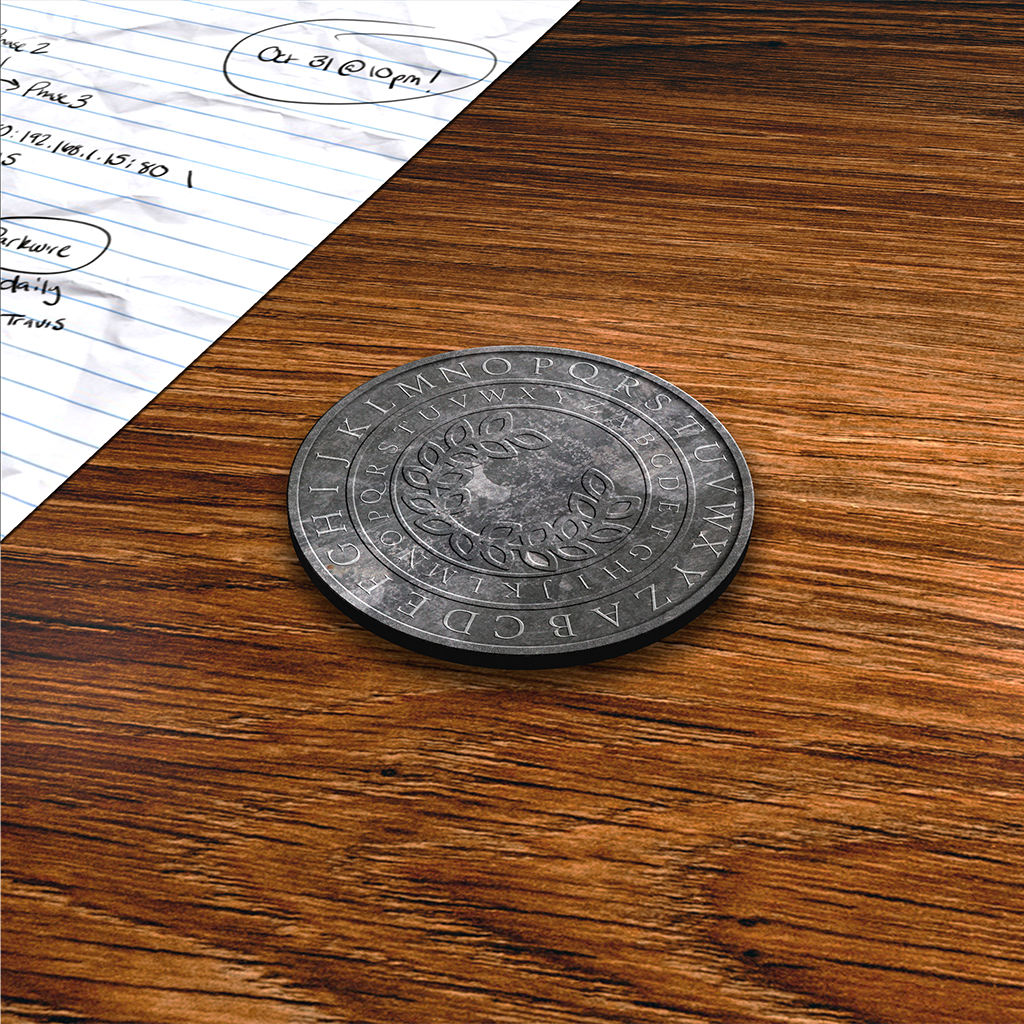
\includegraphics[width=0.6\linewidth]{challenge1.png}
    \caption{Challenge1 image.}
    \label{fig:challenge1}
\end{figure}

% Challenges/Challenge 1/Solution
\subsubsection{Solution}
The original text was encrypted using \textbf{Shift Cipher} technique or also known as \textbf{Caesar Cipher}. It involves replacing each letter in the message by a letter that is some fixed number of positions in the alphabet \cite{Shift Cipher}. The letters are 'shifted' by some number of spaces to the left or right in alphabet. Decryption is performed using reverse direction shifts. This number of spaces/shifts is called \textit{key}. For example, in the case of this challenge, according to the image above it is a right shift of 18 meaning that $key = 18$ and each letter is replaced by a letter which is to the right by 18 positions(e.g. letter S replaces A because it is 18 positions to the right of A's position):
\begin{lstlisting}
Position:          0 1 2 3 4 5 6 7 8 9 . . .          18 19 . . .
Original alphabet: A B C D E F G H I J K L M N O P Q R S T U V W X Y Z
Shifted alphabet:  S T U V W X Y Z A B C D E F G H I J K L M N O P Q R
\end{lstlisting}
Based on this we can decipher the encrypted message:
\begin{lstlisting}
Encrypted text: TGG KUSJWV QGM
Decrypted text: BOO SCARED YOU
\end{lstlisting}
Shift Ciphers work by using the modulo operator to encrypt and decrypt messages performing modulo arithmetic:
\begin{lstlisting}
Encryption: (X + key) mod 26
Decryption: (X - key) mod 26
\end{lstlisting}
Where \textit{X} stands for letter position, '+' shift to the right and '-' shift to the left. Modulo arithmetic is used for the cases when after performing shifts $X<0$ and $X>25$ in order to keep letter position in range 0-25. For example, letter B in the original message was replaced with T: $(1 + 18) \% 26 = 19$. In this case, the decryption can be performed by replacing each letter in ciphertext with the letter which is to the left by 18 positions:
\begin{lstlisting}
TGG KUSJWV QGM
T = 19
(19 - 18) % 26 = 1 | B
G = 6
(6 - 18) % 26 = 14 | O
. . .
\end{lstlisting}
(note: in case of G, after 'shifting', letter position equals -12 which is out of range in alphabet, performing mod 26 letter position becomes one of the number from 0 to 25, in this case 14)
\newline
As a result, the flag is:
\begin{lstlisting}
flag{BOO SCARED YOU}
\end{lstlisting}

%  Challenges/Challenge 2
\subsection{Cryptography: Down the Wrong Path (10 points)}
Flag format:
\begin{lstlisting}
flag{...}
\end{lstlisting}
Description of the challenge is the following:
\begin{tcolorbox}
One of our operatives took a photo of a notebook belonging to Donnell. We think it's a message intended for another member of DEADFACE. Can you decipher the message and tell us who it's intended for?
\end{tcolorbox}
\begin{figure}[H]
    \centering
    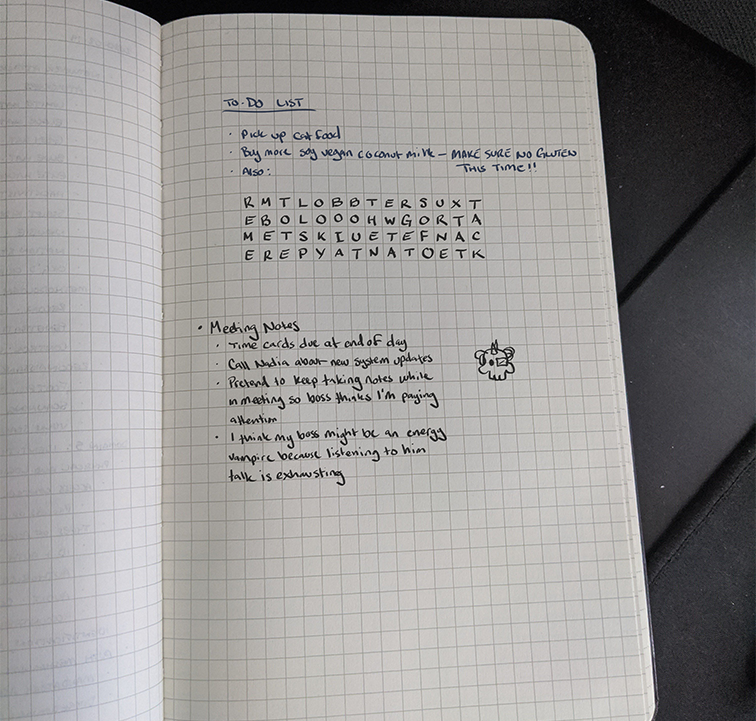
\includegraphics[height=0.55\linewidth]{challenge2.png}
    \caption{Challenge2 image.}
    \label{fig:challenge2}
\end{figure}

% Challenges/Challenge 2/Solution
\subsubsection{Solution}
The original text was encrypted using \textbf{Transposition Cipher} technique, specifically \textbf{Route Cipher}. In \textbf{Transposition Cipher}, the letters are reordered in some way according to a given rule which is called \textit{key}. In a \textbf{Route Cipher} technique, plaintext is written in a grid of given dimensions \cite{Route Cipher2}. One dimension is determined by the key and the second depends on the data size. The plaintext is then read off following the \textit{route} to create a ciphertext, for example \textit{zigzagging up and down}, \textit{spiral inwards clockwise starting from the top right}, etc \cite{Route Cipher1}.
\newline
Based on the image, the message is already constructed in a grid, so there is no need to rearrange different possible grids. The only step remains is to find a right route to read a plaintext. The name of the challenge might be a hint(Down the Wrong Path), so one of the possible ways of reading is \textit{down of the grid}. Next was to select between reading \textit{to the right} or \textit{to the left}. The route was discovered and message is deciphered:
\begin{lstlisting}
|  R M T L O B B T E R A U X T
|  E B O L O O O H W G O R T A
|  M E T S K I U E T E F N A C
v  E R E P Y A T N A T O E T K

REMEMBERTOTELLSPOOKYBOIABOUTTHENEWTARGETSOFOURNEXTATTACK
REMEMBER TO TELL SPOOKY BOI ABOUT THE NEW TARGETS OF OUR NEXT ATTACK
\end{lstlisting}
However, this was not a flag, the challenge required to find out who this message was inteded for. Thus, the flag is:
\begin{lstlisting}
flag{SPOOKYBOI}
\end{lstlisting}

% References
\begin{thebibliography}{10}

    \bibitem{HacktoberCTF Blog}
	HacktoberCTF Official Blog, URL: \url{https://blog.cyberhacktics.com/hacktober-2020/}

	\bibitem{Shift Cipher}
	Caesar cipher, URL: \url{https://en.wikipedia.org/wiki/Caesar_cipher}
	
	\bibitem{Route Cipher1}
	Route Cipher, URL: \url{https://crypto.interactive-maths.com/route-cipher.html}
	
	\bibitem{Route Cipher2}
	Route Cipher, URL: \url{http://www.crypto-it.net/eng/simple/route-cipher.html}
	
\end{thebibliography}

% Appendices
\begin{appendices}

% Screenshots
\section{Screenshots and Writeup links}
\begin{figure}[H]
    \centering
    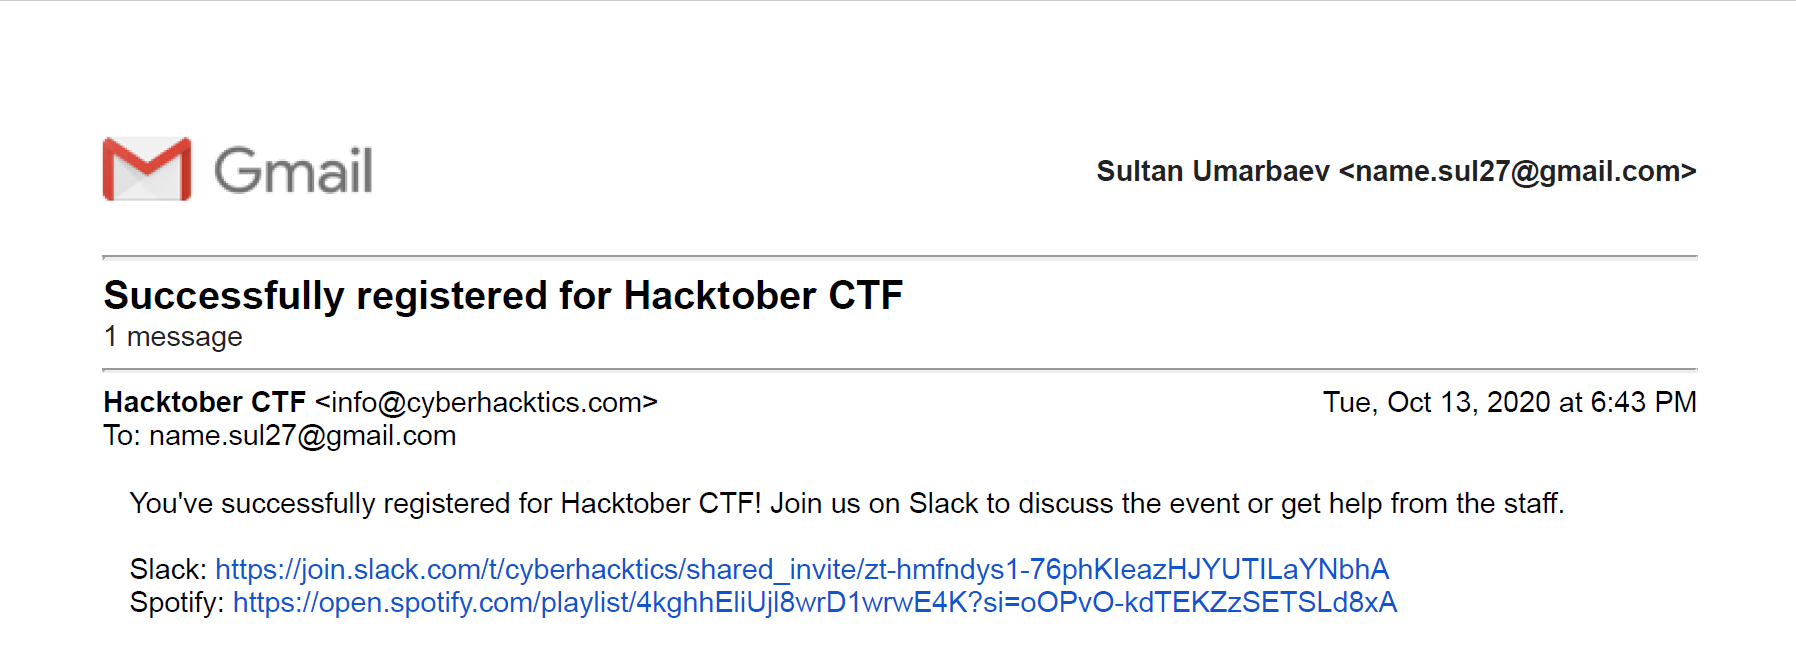
\includegraphics[width=1\linewidth]{Registration_confirmation.png}
    \caption{Confirmation mail from the CTF event.}
    \label{fig:emailconfirmation}
\end{figure}

\begin{figure}[H]
    \centering
    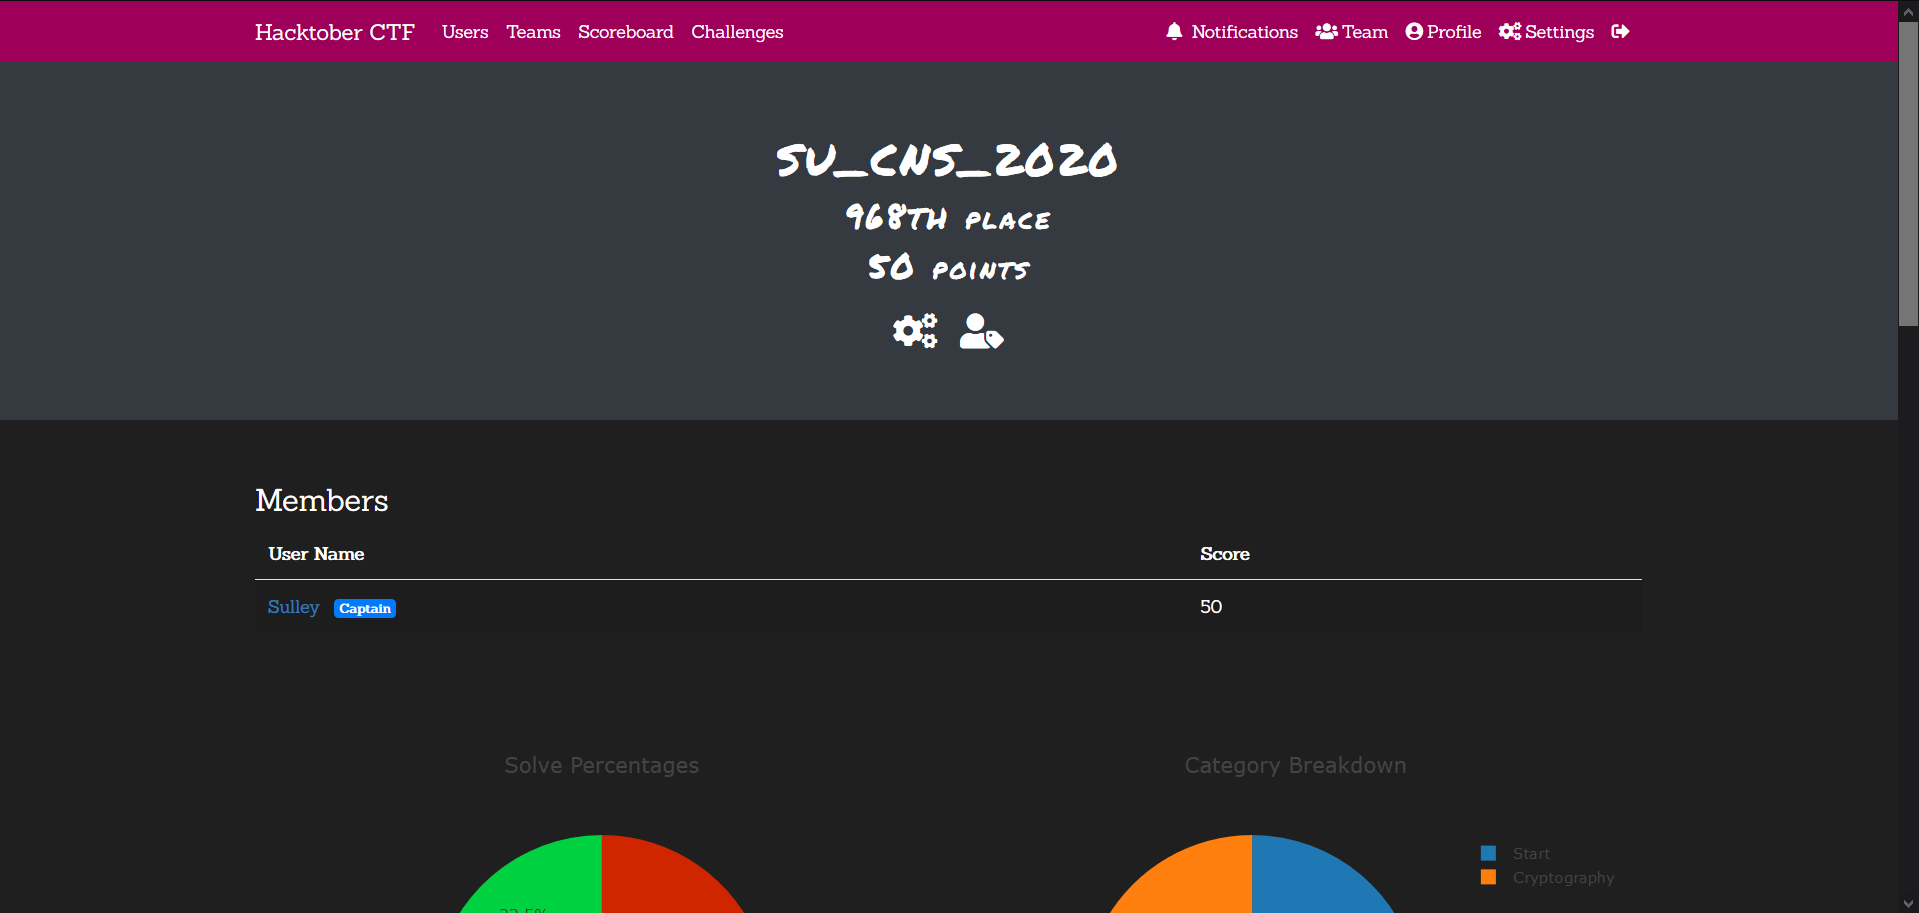
\includegraphics[width=1\linewidth]{Team.png}
    \caption{Team information.}
    \label{fig:teaminfo}
\end{figure}

\begin{figure}[H]
    \centering
    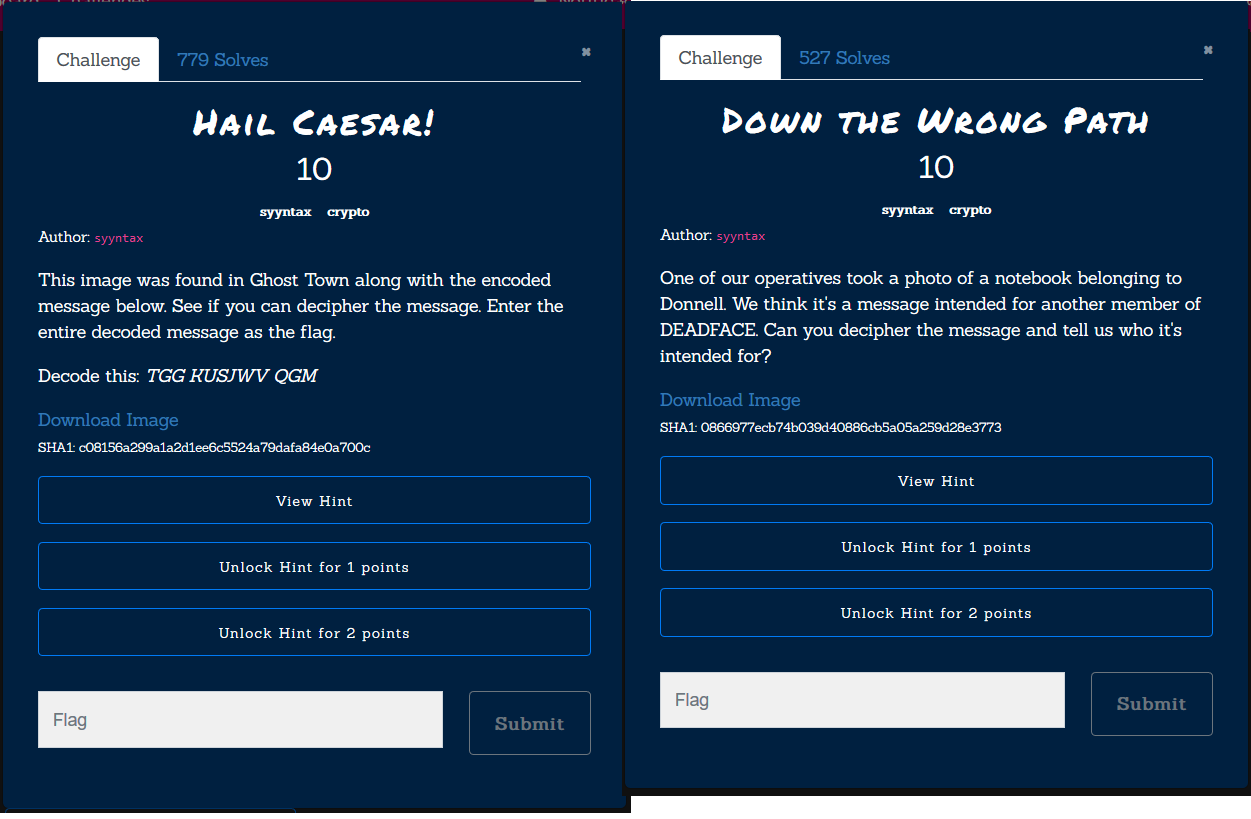
\includegraphics[height=0.5\linewidth]{Challenges_info.png}
    \caption{Descriptions of challenges.}
    \label{fig:challenges}
\end{figure}

\begin{figure}[H]
    \centering
    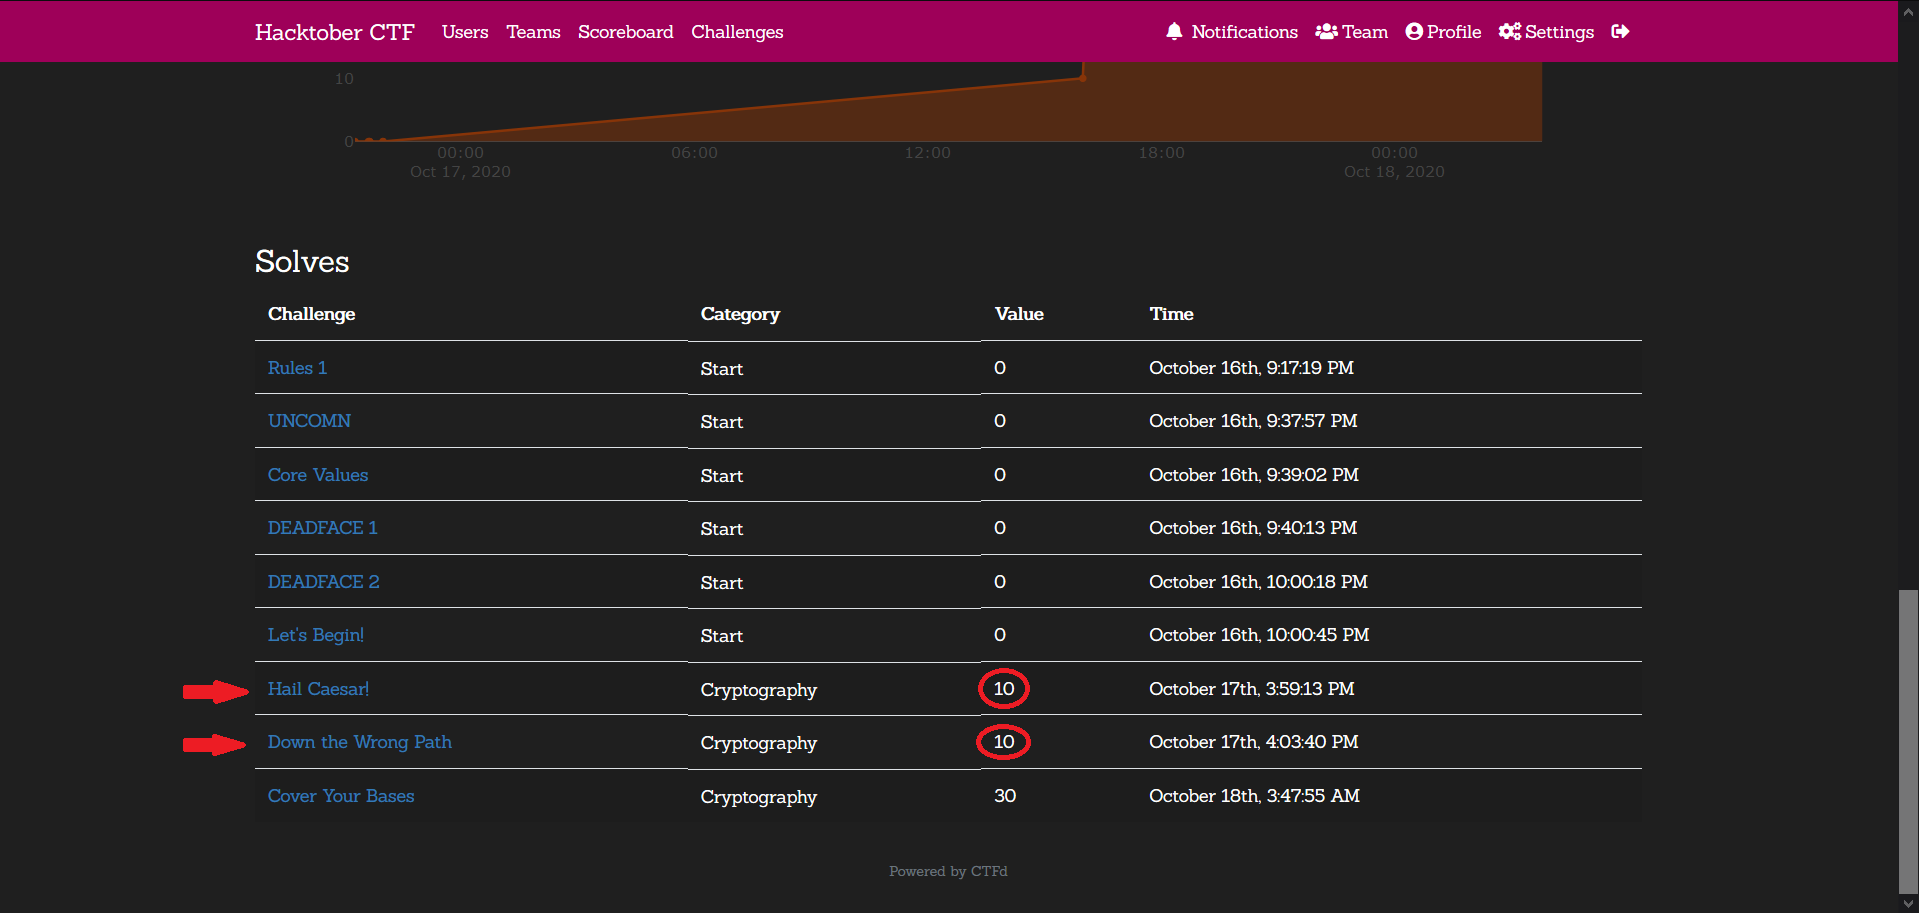
\includegraphics[width=1\linewidth]{Challenge_confirmation.png}
    \caption{Points on the CTF.}
    \label{fig:pointsconfirmation}
\end{figure}

% Links to the writeups
Links to the writeups:
\begin{itemize}
    \item Hail Caesar!, \url{https://ctftime.org/writeup/24273} 
    \item Down the Wrong Path, \url{https://ctftime.org/writeup/24285}
\end{itemize}

% C++ code for Challenge1, Shift Cipher Decryptor 
\section{C++ Code, Shift Cipher Decryptor for Challenge 1}
\begin{listing}[h]
\inputminted{C++}{ShiftCipherDecryptor.cpp}
\caption{Shift Cipher Decryptor.}
\label{listing:scd}
\end{listing}

\end{appendices}

\end{document}
